It is important to draft an overview of the game before starting implementation, just like any other piece of software. The first question is whether the game should be 2D or 3D, as this would result in a vastly different game between the 2 choices, even if the main concepts stay the same. There are also hybrid options, such as Ortographic 3D or 2D gameplay with 3D graphics (also referred to as 2.5D), where 3D-based physics would serve a more aesthetic than functional role. The sample game used and developed in this study is a fully 3D game.\\
Another critically important choice is the genre of the game, which helps define the game world. The game world is where everything happens, it is what the player will see, the objects the player character interacts with and where the scope and purpose of the game exist. Essentially, the game world is to the player character as the real world is to the actual player. Main aspects to consider here would be for example whether the game would be a strategy-based game, in which case the player would control an array of game objects (often referred to as units), or a role-playing / shooting game, where typically the control of a single player character of a time is involved. This also impacts the User Interface within the game, as player controls and game information are closely related to the genre. \\ \\
\begin{figure}
\centering
\begin{subfigure}{0.49\textwidth}
\begin{subfigure}{0.49\textwidth}
\centering
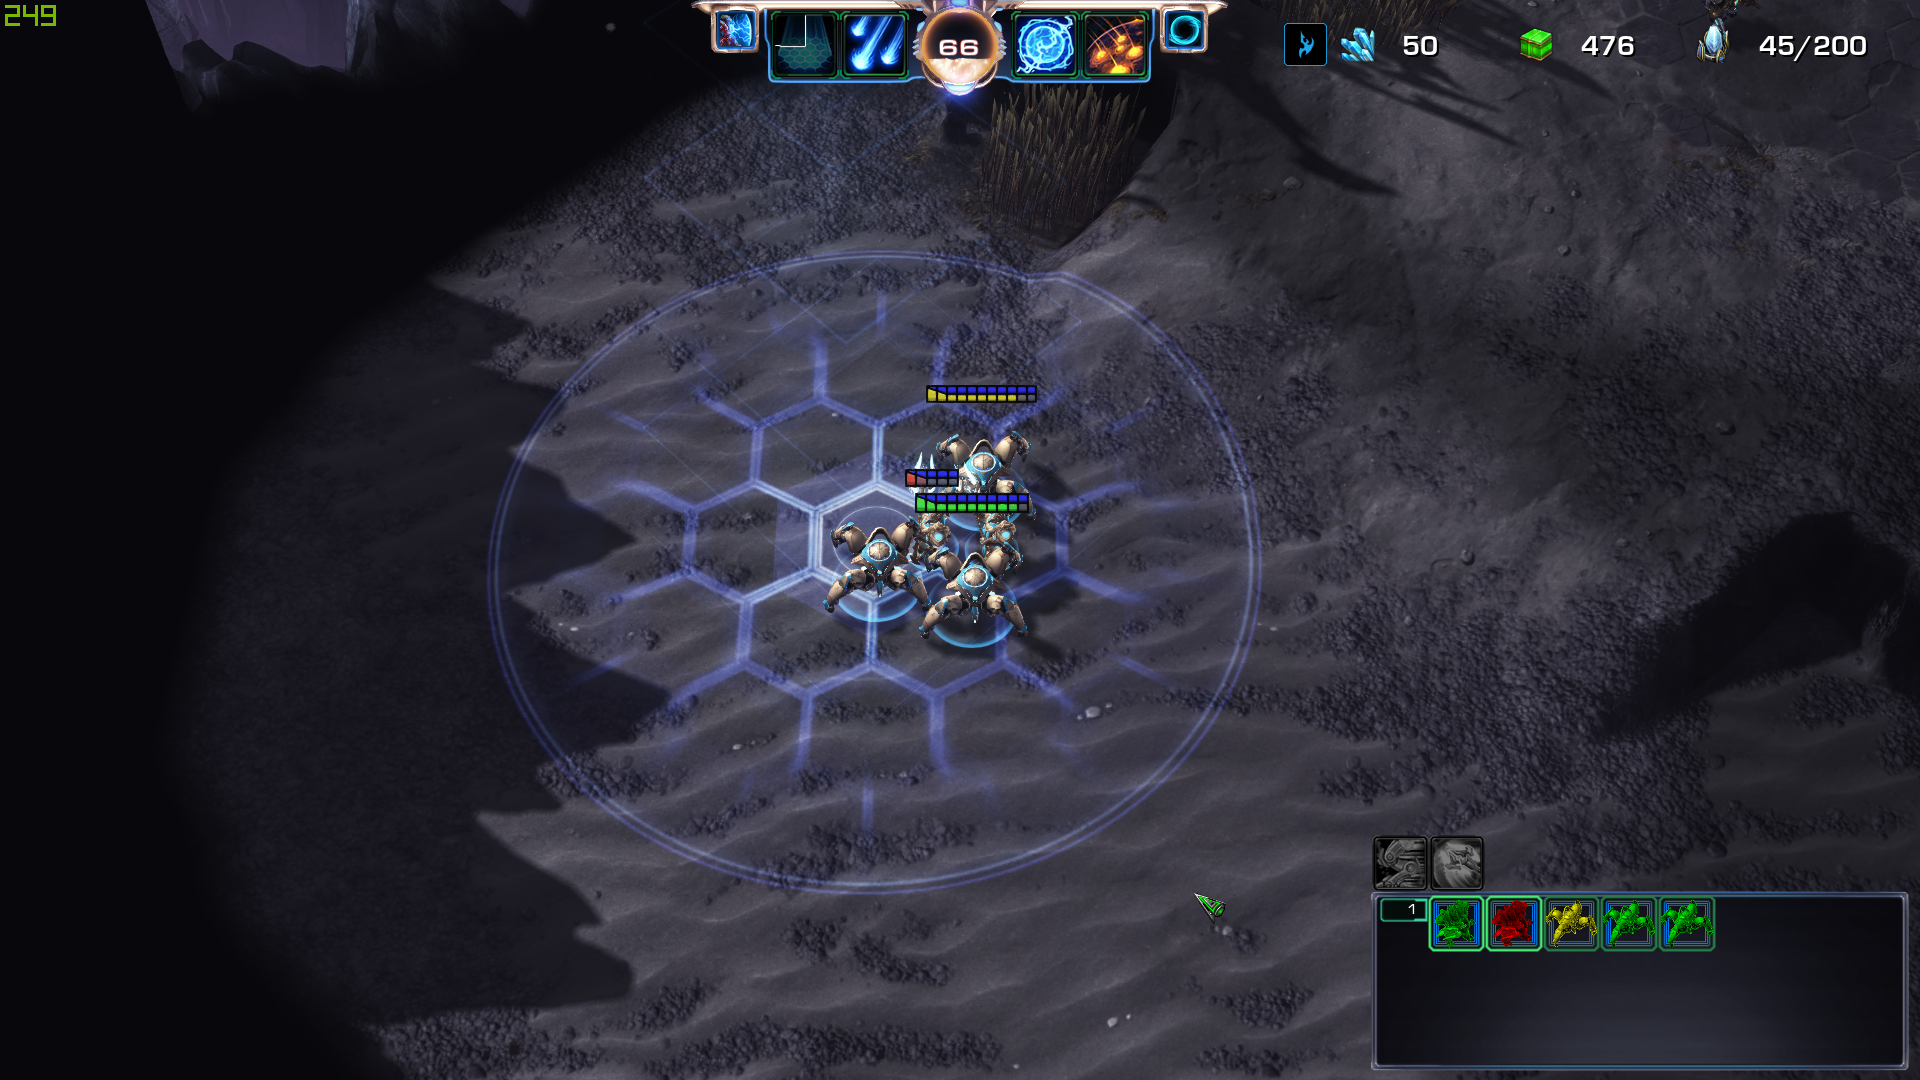
\includegraphics[width = \textwidth, height = 0.66\textwidth]{images/sc2}
\caption{Strategy game - Starcraft II (Blizzard Entertainment)}
\label{fig:left}
\end{subfigure}
\begin{subfigure}{0.49\textwidth}
\centering
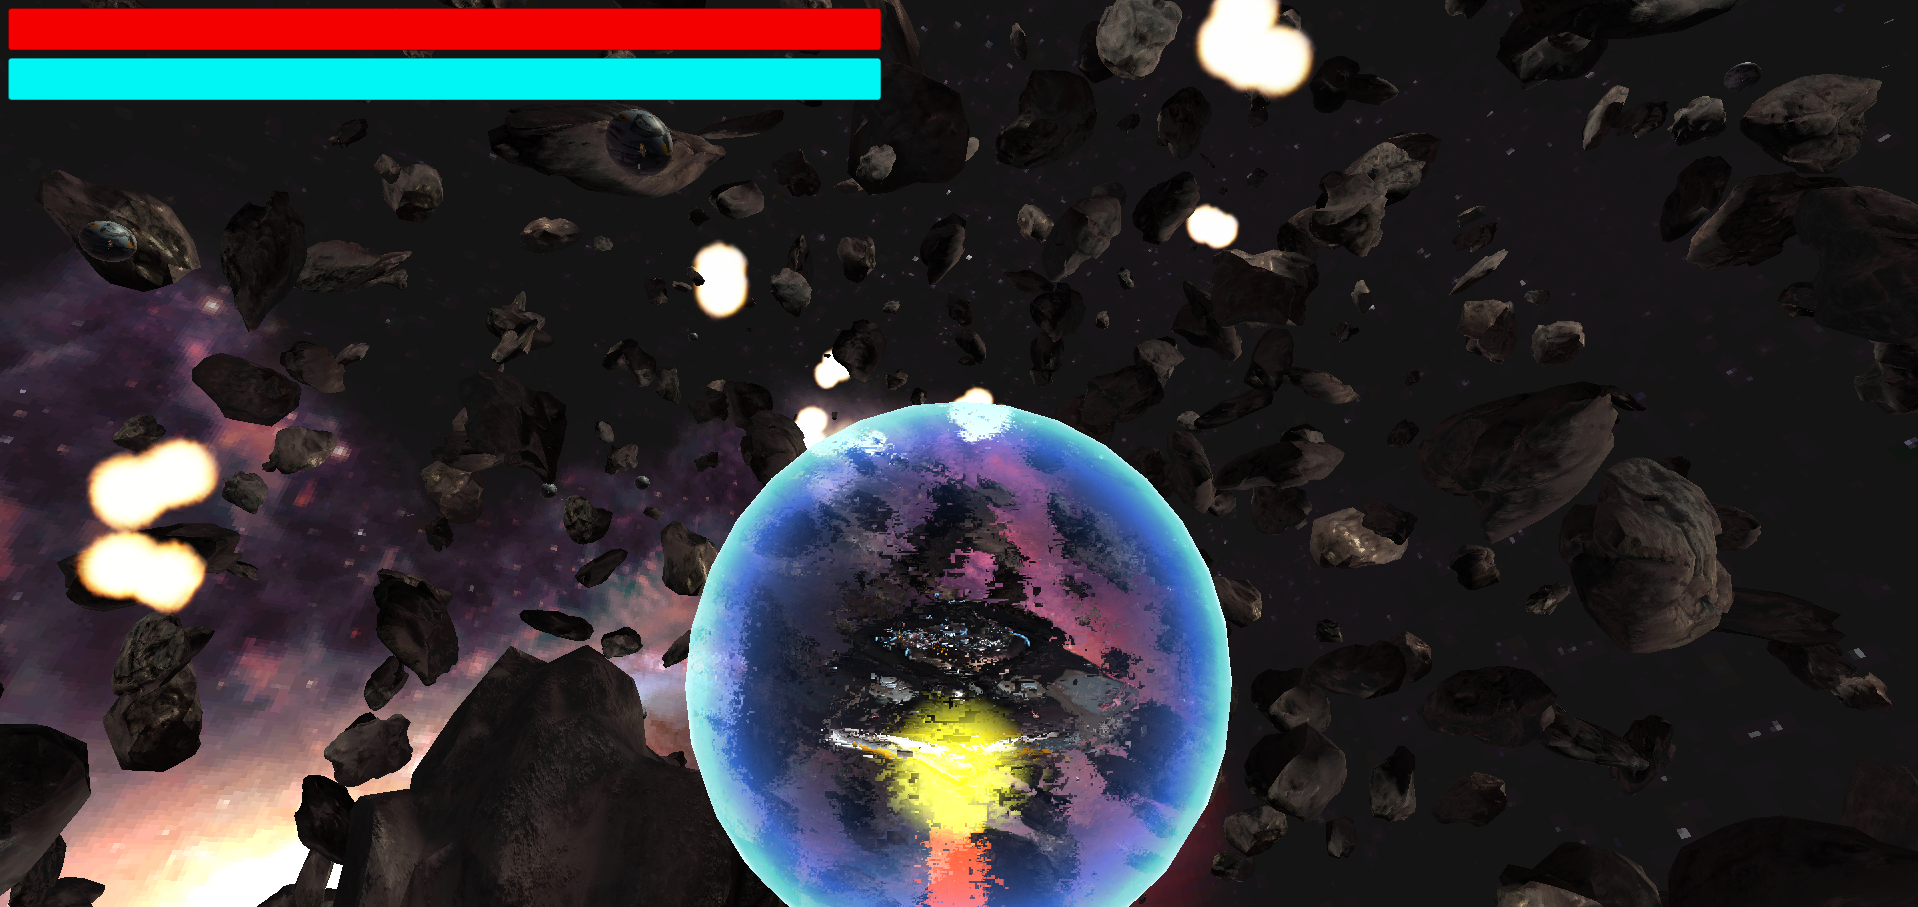
\includegraphics[width = \textwidth, height = 0.66\textwidth]{images/spaceshooter}
\caption{Space Shooter game - sample game}
\label{fig:right}
\end{subfigure}
\end{subfigure}
\caption{Strategy and Shooting genres first impression}
\label{fig:combined}
\end{figure}
In Figure 2.a, an example of a Strategy game is shown. The camera angle is worth noting, as it is not moving along with the controlled game objects, instead it is controlled manually by the player at will. In Figure 2.b, the sample game developed for this paper is shown. The camera cannot be directly controlled, instead it follows the player character, the ship, as it flies around. \\ \\
On paper, the game world is limited by the creator's imagination. In practice however, it is limited by the development possibilities, resources and hardware. Every object present in the game must be modeled (whether 3D or 2D), art, effects, behaviors, animations, everything must be created from scratch. Unity also provides developers with an Asset Stores where content creators can make their works available (free or paid) for others to use, but in the end, everything is made from scratch. The more work and objects are put in the game world, the richer it becomes, but this comes with a penalty in performance. Every object, effect, or behavior comes with its cost, which may be greater or smaller. Once the limit of hardware is reached, compromises must be made, such as limiting the game world in some way, or raising the target hardware performance. Each option has its drawbacks, players may be less interested in a game that doesn't look ``as pretty'', and likewise may not be interested in a game that requires too expensive hardware to be playable. In the strategy genre for example, the mechanic of the player creating more units is often encountered. A limit to the number of units should be implemented, or the game's performance will steadily decrease as more units are added.\\ \\
The player can see the game world through the use of cameras, which render parts of the world, translating a 3D environment (if necessary) to a flat, 2D image. This image can be either displayed on the screen, often called the main camera, or used as a texture for effects such as in-game computer screens displaying other areas of the game world.\\
Textures are essentially object skins. They are wrapped around them, stretching to match certain texture mapping points on them. The end result is a finished object, with the shape of the model and the coloring of the texture, as it is mapped.\\
Another key aspect in a game is the lighting system. Without light, there is nothing to see, resulting in a disappointing experience for the player. Shadows and reflections bring realism, by altering the effect light has on various object to emulate real world effects. In 3D rendering, two major techniques are used: rasterization and ray-tracing. \\
The most widely used is rasteriztion, a highly efficient method that trades fidelity for speed, often with results that fool the user into not noticing the visual anomalies. ``With rasterization, objects on the screen are created from a mesh of virtual triangles, or polygons, that create 3D models of objects. In this virtual mesh, the corners of each triangle — known as vertices — intersect with the vertices of other triangles of different sizes and shapes. A lot of information is associated with each vertex, including its position in space, as well as information about color, texture and its “normal,” which is used to determine the way the surface of an object is facing.
Computers then convert the triangles of the 3D models into pixels, or dots, on a 2D screen. Each pixel can be assigned an initial color value from the data stored in the triangle vertices.
Further pixel processing or “shading,” including changing pixel color based on how lights in the scene hit the pixel, and applying one or more textures to the pixel, combine to generate the final color applied to a pixel.'' \cite{NvidiaRastRT} \\
Another important piece of a well-made Unity game is it's scripting system. The language of choice for them is either Javascript or C\#, the latter being used for the Space Shooter game. Scripts define behaviors and interactions between various game objects, being able to manipulate, create and destroy them.  \\
Player interaction is done through the UI, using buttons, canvases, progress bars, key presses and other similar means. Those components do not directly interact with other game objects, but may have effects on the game world through scripts attached. \\ \\
The vibrancy and the ability to captivate a player lies in the effects, providing immersion. Sound effects played at key moments, particle systems making trail, smoke and explosion effects, all these serve to improve the quality of the player experience, but again, at a cost of performance. Particle systems create many automatically managed, low impact game objects (particles), but when used too often, and with too high particle count, it can affect the smoothness of the gameplay, something undesirable for any player. \\
Unity provides a plethora of features and options, many being outside the scope of this paper. The reader is encouraged to check the Unity official documentation for further study. \cite{unitymanual}